\documentclass[12pt]{article}
\usepackage{standalone}
\usepackage{graphicx}

% Nom du sommaire
\renewcommand*\contentsname{Sommaire}

\begin{document}

% Page de Titre
\begin{titlepage}
    \begin{center}
        \textbf{Rapport de Génie Logiciel} \\
        \vspace{0.5cm}
        Titouan Loiseau et Baptiste Marchand \\
        4A SAGI - TD2 \\
        \vspace{5cm}

        
\includegraphics[height=3cm]{img/Polytech_Angers.png} \\
        
\includegraphics[height=2cm]{img/git.png}
        
\includegraphics[height=2cm]{img/junit.png}
        
\includegraphics[height=2cm]{img/uml.png}
    \end{center}
\end{titlepage}

% Sommaire
\tableofcontents
\pagebreak

% Introduction
\addcontentsline{toc}{section}{Introduction}
\section*{Introduction}

% Exercice 1
\section{Exercice 1}
\subsection{Q1}

La figure~\ref{UC1} présente le premier diagramme de classes imaginé. 

\begin{figure}[h]
    \centering
    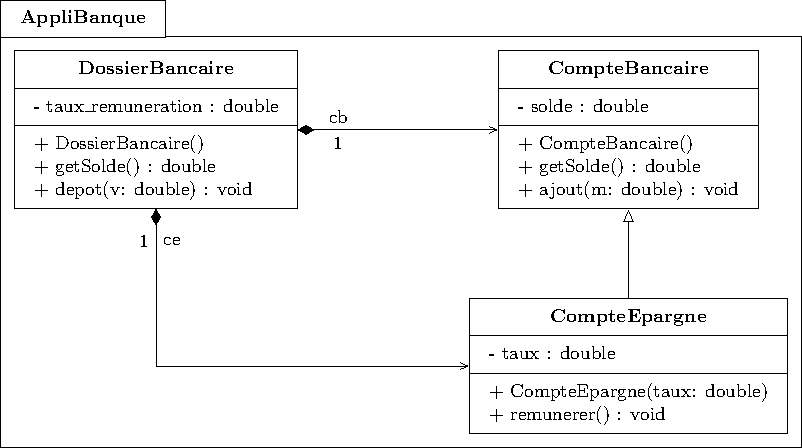
\includegraphics{Diagrammes/UML_UC1.pdf}
    \caption{Diagramme de classes\label{UC1}}
\end{figure}

\newpage 


\subsection{Q2}

La figure~\ref{US1} présente le premier diagramme de classes imaginé. 
\begin{figure}[h]
    \centering
    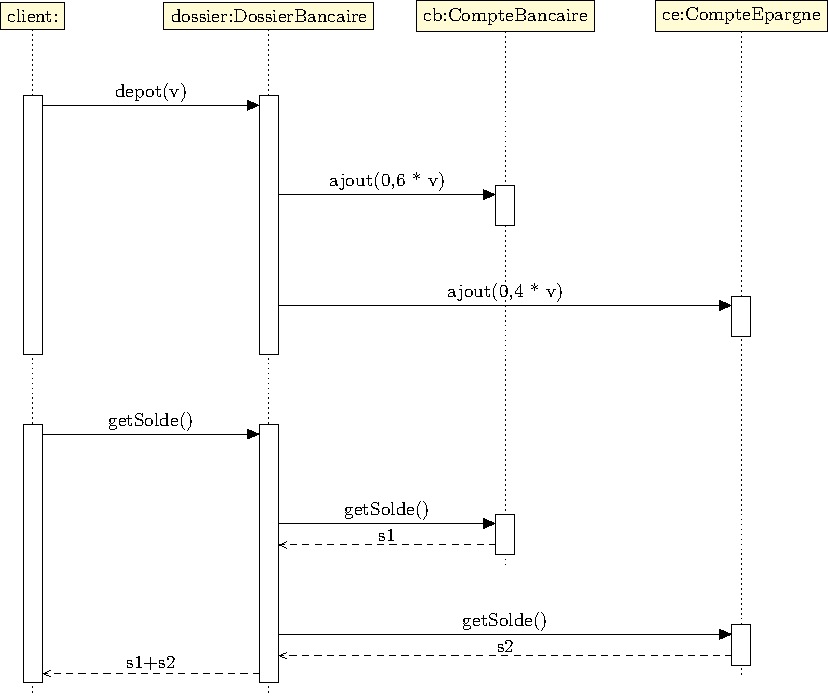
\includegraphics[height=8cm]{Diagrammes/UML_US1.pdf}
    \caption{Diagramme de séquence\label{US1}}
\end{figure}


\subsection{Q3}

En plus des diagrammes précédents, on peut faire un diragramme d'objets modélisant l'état du programme après l'instanciation de l'objet de la classe DossierBancaire.
La figure~\ref{UO1} présente un tel diagramme. 
\begin{figure}[h]
    \centering
    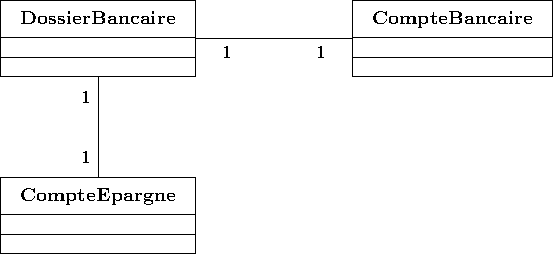
\includegraphics[height=3cm]{Diagrammes/UML_UO1.pdf}
    \caption{Diagramme d\textquotesingle objets\label{UO1}}
\end{figure}

% Exercice 2
\section{Exercice 2}

Pour la compilation du projet simplement, les commandes trouvées 
dans le README permettent de compiler le projet.
\\
Pour la compilation des tests, il faut d'abord télécharger JUnit 4 et hamcrest-core et placer les fichiers .jar
à un endroit connu (l'emplacement du projet par exemple). En utilisant les commandes du README en adaptant les 
chemins en fonction de l'emplacement local, on peut compiler exécuter les tests.

% Exercice 3
\section{Exercice 3}

Pour travailler parallèlement sur le projet, nous avous utilisé le logiciel de versionning git couplé à un outil 
de dépôt en ligne appelé GitHub. Les étapes effectuées pour initialiser le dépôt sont:
\begin{itemize}
    \item Création de l'arboresence des fichiers, avec un dossier "Projet" contenant le code Java, et un dossier "Rapport" contenant le rapport
    \item Ecriture du fichier .gitignore, permettant de ne pas avoir de fichiers inutiles dans le dépôt, notamment le bytecote généré par Java et les fichiers de log de \LaTeX.
    \item Initialisation du dépôt local avec la commande \textquotesingle git init\textquotesingle
    \item Ajout des fichiers à prendre en compte dans le commit avec \textquotesingle git add .\textquotesingle 
    \item Commit la version de départ avec \textquotesingle git commit -m "Commit initial"\textquotesingle 
    \item Création du dépôt distant sur github avec l'utilitaire invoqué par la commande\textquotesingle gh repo create\textquotesingle 
    \item Push du contenu local sur le dépôt distant avec \textquotesingle git push -u origin master\textquotesingle 
\end{itemize}

Par la suite, nous avons effectué les différents commits via la console en ajoutant des tags quand 
nécéssaire avec la commande \textquotesingle git tag\textquotesingle .

\end{document}